\section{Branching takeoff}\label{sec:branching}

\subsection{The tree of improvements}

A self-improving system need not move along a chain. Each kept improvement may spawn several candidates for the next, and the improvements form a tree (Fig.~\ref{fig:branchtree}). The model is a Galton--Watson process with checks.

\begin{definition}[Checked branching process]\label{def:branching}
Generation $0$ is one kept correct system. Each kept correct improvement of generation $k-1$ spawns an independent copy of a random number $\xi\ge0$ of candidates, with $\EE\,\xi=\mu$ and $\PR(\xi\ge1)>0$. Each candidate is correct with probability $\gamma\in(0,1)$, independently. The check of generation $k$ keeps a correct candidate with probability $1-\eta$ and an incorrect one with probability $\delta_{k}\in(0,1]$. Kept incorrect candidates are quarantined: they spawn nothing. Let $Z_{k}$ be the number of kept correct improvements of generation $k$, $F_{k}$ the number of kept incorrect ones, $F=\sum_{k\ge1}F_{k}$, and $m=\mu\gamma(1-\eta)$.
\end{definition}

The number $N$ of kept correct offspring of one kept correct improvement is obtained from $\xi$ by keeping each candidate independently with probability $\gamma(1-\eta)$, so $(Z_{k})$ is a Galton--Watson process with offspring law $N$ and mean $\EE N=m$. If $\xi$ is Poisson with mean $\mu$, then $N$ is Poisson with mean $m$. The quarantine assumption is needed only for the formula for $\EE F$; without it $F$ is larger, so the statements that force $F=\infty$ hold a fortiori.

\begin{figure*}[t]
\centering
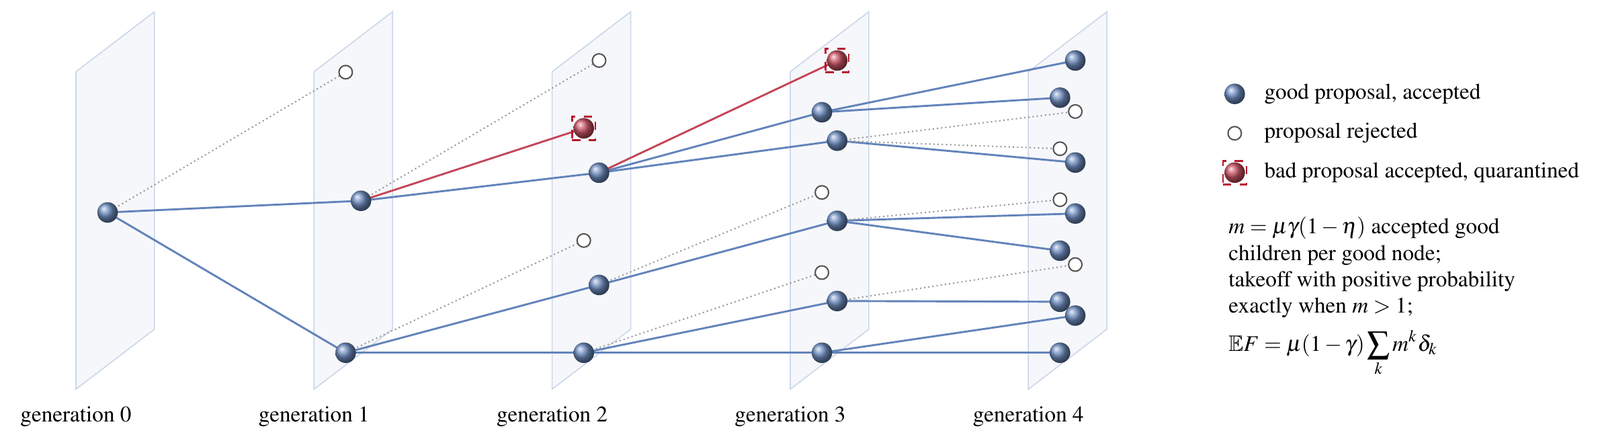
\includegraphics[width=0.92\textwidth]{figures/fig_branchtree}
\caption{A checked branching process, Definition~\ref{def:branching}, over four generations drawn as sheets. Blue nodes are kept correct improvements, which spawn the next generation; grey nodes are rejected candidates; red nodes are incorrect candidates that the check kept, which are quarantined. The kept correct improvements grow like $m^{k}$ in mean, and the expected number of kept errors is $\mu(1-\gamma)\sum_{k}m^{k-1}\delta_{k}$ (Theorem~\ref{thm:F}).}
\label{fig:branchtree}
\end{figure*}

\subsection{Takeoff}

The process \emph{takes off} if $Z_{k}>0$ for every $k$. Let $f(z)=\EE\,z^{N}$ and $q=\PR(\text{takeoff})$.

\begin{proposition}[Takeoff threshold]\label{prop:takeoff}
Assume $\PR(N=1)<1$. Then $q>0$ if and only if $m>1$, and $1-q$ is the least root of $f(z)=z$ in $[0,1]$. If moreover $\EE N^{2}<\infty$ and $m>1$, then
\[
\frac{2(m-1)}{f''(1)}\ \le\ q\ \le\ \frac{2(m-1)}{f''(1-q)} .
\]
For Poisson offspring, $f''(1)=m^{2}$, $f''(1-q)=m^{2}(1-q)$ and, for $1<m\le2$, $\bigl|q-2(m-1)/m^{2}\bigr|\le4e^{4}(m-1)^{2}$.
\end{proposition}

\begin{proof}
The first two claims are the classical extinction theorem \cite{AN72,WG75}; Appendix~\ref{app:gw} recalls the proof. For the bounds, Taylor's formula at $1$ with $f(1)=1$ and $f'(1)=m$ gives $f(1-q)=1-mq+\frac12f''(\xi)q^{2}$ for some $\xi\in(1-q,1)$. Since $f(1-q)=1-q$, this is $(m-1)q=\frac12f''(\xi)q^{2}$, so $q=2(m-1)/f''(\xi)$; and $f''$ is increasing on $[0,1]$, being a power series with nonnegative coefficients, so $f''(1-q)\le f''(\xi)\le f''(1)$. For Poisson offspring $f(z)=e^{m(z-1)}$, $f''(z)=m^{2}e^{m(z-1)}$, and $e^{-mq}=1-q$ at the fixed point. The two bounds then differ by $\frac{2(m-1)}{m^{2}}\cdot\frac{q}{1-q}$. Extinction has probability at least $\PR(N=0)=e^{-m}\ge e^{-2}$, so $1-q\ge e^{-2}$ and $q\le2e^{2}(m-1)$; the difference is at most $2(m-1)e^{2}\cdot2e^{2}(m-1)$.
\end{proof}

Near the threshold the probability of takeoff is linear in $m-1$, with slope $2/f''(1)$, which tends to $2/\sigma^{2}$ at criticality, $\sigma^{2}$ the variance of the offspring law there; Table~\ref{tab:gw} gives the numbers for Poisson offspring and Fig.~\ref{fig:branching}(a) the curves. A takeoff is never certain: for $m\le2$ it fails with probability at least $e^{-2}$, and it is a matter of luck in its first generations.

\begin{table}[b]
\caption{Probability $q$ of takeoff for Poisson offspring of mean $m$, with the two bounds of Proposition~\ref{prop:takeoff}.}
\label{tab:gw}
\centering
\small
\begin{tabular}{@{}c c c c@{}}
\toprule
$m$ & $2(m-1)/m^{2}$ & $q$ & $2(m-1)/(m^{2}(1-q))$ \\
\midrule
$1.02$ & $0.0385$ & $0.0390$ & $0.0400$ \\
$1.05$ & $0.0907$ & $0.0937$ & $0.1001$ \\
$1.10$ & $0.1653$ & $0.1761$ & $0.2006$ \\
$1.20$ & $0.2778$ & $0.3137$ & $0.4048$ \\
$1.50$ & $0.4444$ & $0.5828$ & $1.0653$ \\
$2.00$ & $0.5000$ & $0.7968$ & $2.4608$ \\
\bottomrule
\end{tabular}
\end{table}

\subsection{Errors in a takeoff}

\begin{proof}[Proof of Theorem~\ref{thm:F}]
\emph{Threshold.} This is Proposition~\ref{prop:takeoff}.

\emph{Expected errors.} Let $\mathcal F_{k}$ be the information of generations $0,\dots,k$. Given $\mathcal F_{k-1}$, the $Z_{k-1}$ kept correct improvements spawn on average $\mu Z_{k-1}$ candidates, each incorrect and kept with probability $(1-\gamma)\delta_{k}$, so $\EE[F_{k}\mid\mathcal F_{k-1}]=\mu(1-\gamma)\delta_{k}Z_{k-1}$. With $\EE Z_{k-1}=m^{k-1}$ and monotone convergence, $\EE F=\mu(1-\gamma)\sum_{k\ge1}m^{k-1}\delta_{k}$. If the series converges, $F<\infty$ almost surely.

\emph{Divergence.} Let $m>1$, $\EE\,\xi\log\xi<\infty$ and $\sum m^{k-1}\delta_{k}=\infty$. Since $N\le\xi$, also $\EE N\log N<\infty$, and the Kesten--Stigum theorem \cite{KS66,AN72} gives $Z_{k}/m^{k}\to W$ almost surely with $W>0$ almost surely on takeoff. Let $B_{k}=\{F_{k}\ge1\}\in\mathcal F_{k}$ and $u_{k}=(1-\gamma)\delta_{k}$. Given $\mathcal F_{k-1}$ the parents act independently, and one parent with $\xi$ candidates keeps no incorrect one with probability $\EE(1-u_{k})^{\xi}\le1-u_{k}\PR(\xi\ge1)$, because $1-(1-u)^{j}\ge u$ for $j\ge1$. With $c_{0}=\PR(\xi\ge1)>0$,
\[
\begin{aligned}
\PR(B_{k}\mid\mathcal F_{k-1})&\ \ge\ 1-(1-c_{0}u_{k})^{Z_{k-1}}\ \ge\ 1-e^{-c_{0}u_{k}Z_{k-1}}\\
&\ \ge\ \tfrac12\min(c_{0}u_{k}Z_{k-1},1),
\end{aligned}
\]
the last step by $1-e^{-x}\ge\frac12\min(x,1)$. On takeoff, $Z_{k-1}\ge\frac12Wm^{k-1}$ for all large $k$, so up to finitely many terms
\[
\sum_{k}\PR(B_{k}\mid\mathcal F_{k-1})\ge\frac12\sum_{k}\min\Bigl(\frac{c_{0}(1-\gamma)W}{2}\,m^{k-1}\delta_{k},\,1\Bigr).
\]
 The right side diverges, since $\sum m^{k-1}\delta_{k}$ diverges and a series $\sum\min(cx_{k},1)$ with $c>0$, $x_{k}\ge0$ converges only if $\sum x_{k}$ does. L\'evy's conditional Borel--Cantelli lemma \cite{Dur19} states that $\{B_{k}\text{ infinitely often}\}$ and $\{\sum_{k}\PR(B_{k}\mid\mathcal F_{k-1})=\infty\}$ agree up to a null set (Appendix~\ref{app:levy}). So $F=\infty$ almost surely on takeoff.

\emph{Exponential checks.} With $\delta_{k}=\eps^{r_{k}}$ and $r_{k}=\lceil k\log(2m)/L\rceil$, $r_{k}L\ge k\log(2m)$, so $m^{k}\eps^{r_{k}}\le2^{-k}$ and $\sum m^{k-1}\delta_{k}\le\frac1m\sum2^{-k}<\infty$. Conversely, if $\sum m^{k-1}\eps^{r_{k}}<\infty$, its terms tend to $0$, so $r_{k}L-(k-1)\log m\to\infty$, hence $r_{k}L\ge k\log m$ for all large $k$. A constant $\delta_{k}=\delta>0$ gives $\sum m^{k-1}\delta=\infty$ for $m\ge1$.
\end{proof}

\begin{corollary}[The entropy tax of a takeoff]\label{cor:branchtax}
In a sound takeoff with exponential checks and $m>1$, every kept correct improvement of generation $k$ has been checked by at least $k\log m/L=\log(\EE Z_{k})/L$ runs, for all large $k$.
\end{corollary}

The tax is the logarithm of the size of the population, divided by $L$, exactly as for $n$ candidates of equal cost in Corollary~\ref{cor:uniform}: a growing population of improvements can stay sound only if each new improvement is checked harder than the last by a fixed number of runs per generation, and a fixed false acceptance rate, however small, lets errors multiply with the population (Fig.~\ref{fig:branching}(b)).

\begin{figure*}[t]
\centering
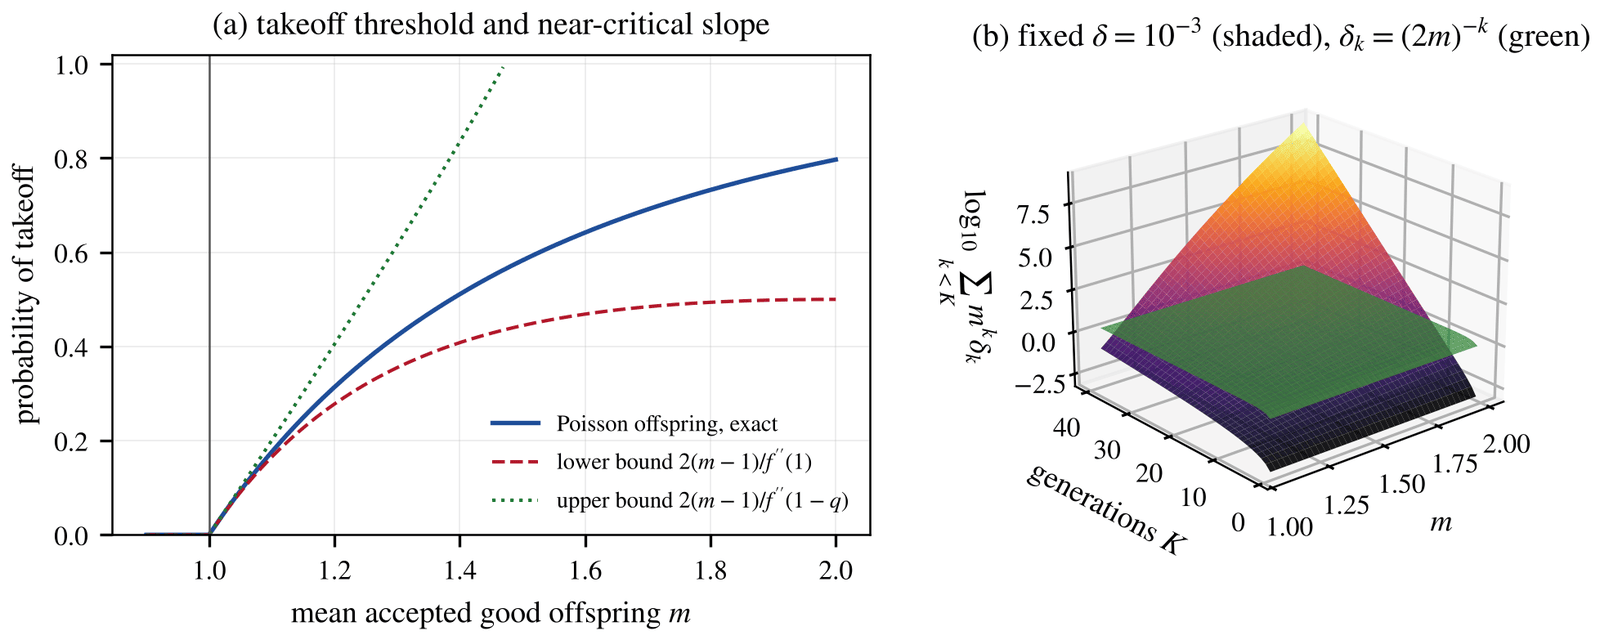
\includegraphics[width=0.98\textwidth]{figures/fig_branching}
\caption{Theorem~\ref{thm:F}. (a) The probability of takeoff for Poisson offspring as a function of the mean $m$ of kept correct offspring, with the two bounds of Proposition~\ref{prop:takeoff}; the threshold is $m=1$ and the slope there is $2$. (b) The expected number of kept errors in the first $K$ generations, $\log_{10}\sum_{k<K}m^{k}\delta_{k}$, for a fixed rate $\delta=10^{-3}$ (shaded surface), which grows without bound, and for the amplified rate $\delta_{k}=(2m)^{-k}$ (green), which stays below $\log_{10}2$.}
\label{fig:branching}
\end{figure*}
